\section{Results}\label{sec:results}

\subsection{Correctness}\label{subsec:res-correctness}

Table~\ref{tab:correctness} summarises the comparison of every reported instance with the independent reference
(Section~\ref{subsec:metrics}). All \NumCorrectnessInstances~checked instances, from $n=\NumCorrectnessNmin$ to
$n=\NumCorrectnessNmax$ on one, two and four cards, \NumCorrectnessHaar~of them from Haar random input states, agree with the
reference to double precision rounding: the largest amplitude error is \NumWorstMaxAbsErr\ and the largest infidelity
$1-F$ is \NumWorstOneMinusF. In \NumCorrectnessExact~instances the state is bit identical to the reference. The engine keeps every gate matrix in
float64; the baseline design transfers gate angles as float32 and widens them in the kernel. Its largest amplitude
error is \NumBaselineExactErrMax\ for QFT, GHZ and Bell states from $\ket{0\dots0}$, where no rotation angle affects the
result (in the QFT every controlled phase acts while its control qubit is still $\ket{0}$), but \NumBaselineRotErrMax\ for
random circuits, Grover search and Haar random inputs, whose rotations change the state. Grover search with $k_{\mathrm{opt}}$ iterations
(Table~\ref{tab:grover}) reaches the analytic target probability $\sin^2((2k_{\mathrm{opt}}+1)\theta)$ to within
\NumGroverWorstPdiff. The counting registers of the phase estimation runs (order finding for $N=15$ and phase estimation
of $P(2\pi\phi)$, rows shor15 and qpe of Table~\ref{tab:correctness}) reproduce the probability distribution of the
reference to within \NumQpeWorstDistDiff~in every outcome.

\begin{table}[t]
\caption{Correctness of the engine: worst values over all instances of each circuit family, after optimal
global phase alignment. Instances: every width and card count of the campaign; zero input $\ket{0\dots0}$ or Haar random.}\label{tab:correctness}
% generated by scripts/make_tables.py, do not edit
\begin{tabular}{@{}llcrrrr@{}}
\toprule
Circuit & Input & $n$ & Instances & max $1-F$ & max $|\Delta\alpha|$ & max $\ell_2$ \\
\midrule
bell & zero & 4 to 22 & 10 & $1.23\times 10^{-32}$ & $1.11\times 10^{-16}$ & $1.11\times 10^{-16}$ \\
ghz & haar & 12 to 28 & 5 & $3.88\times 10^{-32}$ & $6.99\times 10^{-18}$ & $1.97\times 10^{-16}$ \\
ghz & zero & 4 to 30 & 22 & $1.23\times 10^{-32}$ & $1.11\times 10^{-16}$ & $1.11\times 10^{-16}$ \\
grover & zero & 4 to 6 & 2 & $2.12\times 10^{-29}$ & $1.30\times 10^{-15}$ & $4.60\times 10^{-15}$ \\
partition heavy & haar & 12 to 28 & 5 & $8.50\times 10^{-31}$ & $3.38\times 10^{-17}$ & $9.22\times 10^{-16}$ \\
partition heavy & zero & 4 to 22 & 10 & $4.19\times 10^{-31}$ & $3.72\times 10^{-16}$ & $6.47\times 10^{-16}$ \\
qft & haar & 12 to 28 & 5 & $1.08\times 10^{-30}$ & $2.36\times 10^{-17}$ & $1.04\times 10^{-15}$ \\
qft & zero & 4 to 30 & 19 & $3.96\times 10^{-30}$ & $8.67\times 10^{-19}$ & $1.99\times 10^{-15}$ \\
qft iqft & zero & 4 to 22 & 10 & $1.82\times 10^{-30}$ & $3.33\times 10^{-16}$ & $1.35\times 10^{-15}$ \\
rand10 & haar & 12 to 28 & 5 & $3.83\times 10^{-30}$ & $6.14\times 10^{-17}$ & $1.96\times 10^{-15}$ \\
rand10 & zero & 4 to 22 & 10 & $2.76\times 10^{-30}$ & $2.39\times 10^{-16}$ & $1.66\times 10^{-15}$ \\
\bottomrule
\end{tabular}

\end{table}

\begin{table}[t]
\caption{Grover search with $k_{\mathrm{opt}}$ iterations on four cards: measured target probability against
$P(k_{\mathrm{opt}}) = \sin^2((2k_{\mathrm{opt}}+1)\theta)$.}\label{tab:grover}
% generated by scripts/make_tables.py, do not edit
\begin{tabular}{@{}rrrrr@{}}
\toprule
$n$ & $k_{\mathrm{opt}}$ & $P(k)$ analytic & $P$ measured & difference \\
\midrule
4 & 3 & 0.961319 & 0.961319 & $7.66\times 10^{-15}$ \\
6 & 6 & 0.996586 & 0.996586 & $1.87\times 10^{-14}$ \\
8 & 12 & 0.999947 & 0.999947 & $4.55\times 10^{-14}$ \\
10 & 25 & 0.999461 & 0.999461 & $1.11\times 10^{-13}$ \\
12 & 50 & 0.999945 & 0.999945 & $2.55\times 10^{-13}$ \\
14 & 100 & 1.000000 & 1.000000 & $5.80\times 10^{-13}$ \\
16 & 201 & 0.999988 & 0.999988 & $1.31\times 10^{-12}$ \\
\bottomrule
\end{tabular}

\end{table}

\subsection{Largest simulated width}\label{subsec:res-maxwidth}

\begin{table}[t]
\caption{Largest width verified against the reference per number of cards and circuit, HBM occupied per card by the
state, end to end time (median of the timed repetitions; n/a for the single validation runs) and the largest amplitude
error.}\label{tab:maxwidth}
% generated by scripts/make_tables.py, do not edit
\begin{tabular}{@{}rlrrrr@{}}
\toprule
Cards & Circuit & largest $n$ & HBM per card (GiB) & $T_{\mathrm{e2e}}$ (s) & max $|\Delta\alpha|$ \\
\midrule
1 & ghz & 29 & 8 & n/a & $1.11\times 10^{-16}$ \\
1 & qft & 29 & 8 & n/a & $1.02\times 10^{-19}$ \\
1 & rand10 & 28 & 4 & 21.9 & $6.10\times 10^{-19}$ \\
2 & ghz & 30 & 8 & n/a & $1.11\times 10^{-16}$ \\
2 & qft & 30 & 8 & n/a & $7.12\times 10^{-20}$ \\
2 & rand10 & 28 & 2 & n/a & $5.22\times 10^{-19}$ \\
4 & ghz & 31 & 8 & 13.7 & $1.11\times 10^{-16}$ \\
4 & qft & 31 & 8 & 60.8 & $5.42\times 10^{-20}$ \\
4 & qft iqft & 28 & 1 & 20.8 & $7.38\times 10^{-17}$ \\
4 & rand10 & 29 & 2 & 31.1 & $4.16\times 10^{-19}$ \\
\bottomrule
\end{tabular}

\end{table}

\begin{table}[t]
\caption{Instances stopped by the thermal guard (a card reached 90\,\textdegree C FPGA or 85\,\textdegree C HBM): setting of
the slice paths, completed repetitions, the card and its temperatures at the stop. The paths column gives F1, F2, F3 and
F4 in this order (1 on, 0 off, a: F4 chosen by the compiler, Section~\ref{subsec:compilation}).}\label{tab:thermal}
% generated by scripts/make_tables.py, do not edit
\begin{tabular}{@{}rlrlrrr@{}}
\toprule
Cards & Circuit & $n$ & paths & repetitions & card & FPGA / HBM (C) \\
\midrule
4 & qft & 28 & 0000 & 4 of 6 & 21 & 90 / 85 \\
4 & rand10 & 8 & 111a & 1 of 3 & 21 & 93 / 88 \\
4 & grover & 16 & 111a & 5 of 6 & 21 & 90 / 85 \\
4 & qft iqft & 24 & 111a & 0 of 6 & 21 & 90 / 85 \\
4 & qft & 31 & 111a & 2 of 2 & 21 & 91 / 86 \\
4 & qft & 30 & 111a & 3 of 4 & 21 & 90 / 85 \\
4 & ghz & 31 & 111a & 0 of 1 & 21 & 90 / 85 \\
\bottomrule
\end{tabular}

\end{table}

The capacity follows from the memory layout. Every HBM buffer of a slice lies in one pseudo channel of 512~MiB and
holds the slice together with the engine's instruction segment of 4~MiB. For the widest states each card has
\NumPcsUsedFlagship~slices, one per PC, of at most $2^{24}$ amplitudes (256~MiB), so one card holds $n=29$, two cards
$n=30$ and four cards $n=31$. The verified widths reach this capacity on every configuration: \NumMaxWidthOneCard,
\NumMaxWidthTwoCards~and \NumMaxWidthFourCards~qubits (Table~\ref{tab:maxwidth}). The state then takes 8~GiB of the
16~GiB of each card, spread over all 32 pseudo channels. The next power of two, $2^{25}$ amplitudes, would fill a pseudo
channel completely and leave no room for the instruction segment that shares the buffer, so the engine reaches every
pseudo channel but fills only half of the HBM (Section~\ref{sec:limitations}). At $n=31$ GHZ
preparation and the QFT run on the four cards in \NumMaxThirtyOneGhzS~s and \NumMaxThirtyOneQftS~s and agree with the
reference computed by Qiskit Aer. Earlier attempts at this width were stopped by the thermal guard of one card
(Table~\ref{tab:thermal}).

\subsection{FPGA resources}\label{subsec:res-resources}

Table~\ref{tab:resources} gives the post route utilisation of both bitstreams. The baseline kernel occupies
\NumLutPctVsix\,\% of the LUTs, \NumDspPctVsix\,\% of the DSPs and \NumBramPctVsix\,\% of the BRAM and closes timing at
\NumClockVsix~MHz. The engine build with \NumEnginesFlagship~compute units uses \NumLutPctFlagship\,\% of the LUTs,
\NumDspPctFlagship\,\% of the DSPs, \NumBramPctFlagship\,\% of the BRAM tiles and \NumUramPctFlagship\,\% of the URAM at \NumClockFlagship~MHz. The DSPs
implement the double precision arithmetic of the $2\times2$ primitive. The build with sixteen compute units placed but
failed in routing (Section~\ref{subsec:engine}), so the engine count is limited by routing congestion rather than by the
number of LUTs or DSPs. The PC bindings of both builds are
given in Sections~\ref{subsec:baseline-design} and~\ref{subsec:engine}.

\begin{table}[t]
\caption{Post route utilisation (full device including the shell) and achieved kernel clock of the bitstreams
used in this paper.}\label{tab:resources}
% generated by scripts/make_tables.py, do not edit
\begin{tabular}{@{}lrrrrrr@{}}
\toprule
Build & MHz & LUT (\%) & FF (\%) & DSP (\%) & BRAM tiles (\%) & URAM (\%) \\
\midrule
baseline (8 data ports) & 258 & 209{,}980 (16.1) & 250{,}174 (9.6) & 727 (8.1) & 238 (11.8) & 0 (0.0) \\
engine, 8 compute units & 300 & 486{,}506 (37.3) & 684{,}497 (26.2) & 2{,}692 (29.8) & 808 (40.1) & 64 (6.7) \\
engine, 16 compute units & \multicolumn{6}{l}{placed; routing failed (conflicted nets)} \\
device total (XCU55C) & & 1{,}303{,}680 & 2{,}607{,}360 & 9{,}024 & 2{,}016 & 960 \\
\bottomrule
\end{tabular}

\end{table}

\subsection{Where the time goes}\label{subsec:res-breakdown}

\begin{table}[t]
\caption{Routing of the engine on four cards (compiler counters). ``gates'' counts the gates of the circuit; the
following columns count operations after fusion of consecutive single qubit gates and absorption of SWAP gates into the
qubit map, so they do not add up to the gate count: local operations, partition controlled (F2), partition diagonal (F1),
slice relabelling (F3) and operations that required a remap; then remaps and HBM passes.}\label{tab:routing}
% generated by scripts/make_tables.py, do not edit
\begin{tabular}{@{}lrrrrrrrrr@{}}
\toprule
Circuit & $n$ & gates & local & F2 & F1 & F3 & exchange & remaps & passes \\
\midrule
bell & 20 & 2 & 1 & 0 & 0 & 0 & 1 & 1 & 2 \\
ghz & 20 & 20 & 15 & 1 & 0 & 3 & 1 & 1 & 4 \\
ghz & 28 & 28 & 23 & 1 & 0 & 3 & 1 & 1 & 6 \\
partition heavy & 20 & 40 & 15 & 0 & 0 & 0 & 2 & 2 & 2 \\
qft & 20 & 220 & 116 & 55 & 31 & 0 & 8 & 8 & 24 \\
qft & 28 & 420 & 268 & 85 & 44 & 0 & 9 & 9 & 76 \\
qft iqft & 20 & 460 & 258 & 153 & 6 & 0 & 21 & 21 & 59 \\
qft iqft & 28 & 868 & 563 & 244 & 8 & 0 & 23 & 23 & 169 \\
rand10 & 20 & 300 & 279 & 0 & 0 & 0 & 21 & 21 & 29 \\
rand10 & 28 & 420 & 400 & 0 & 0 & 0 & 20 & 20 & 46 \\
\bottomrule
\end{tabular}

\end{table}

\begin{figure}[t]
\centering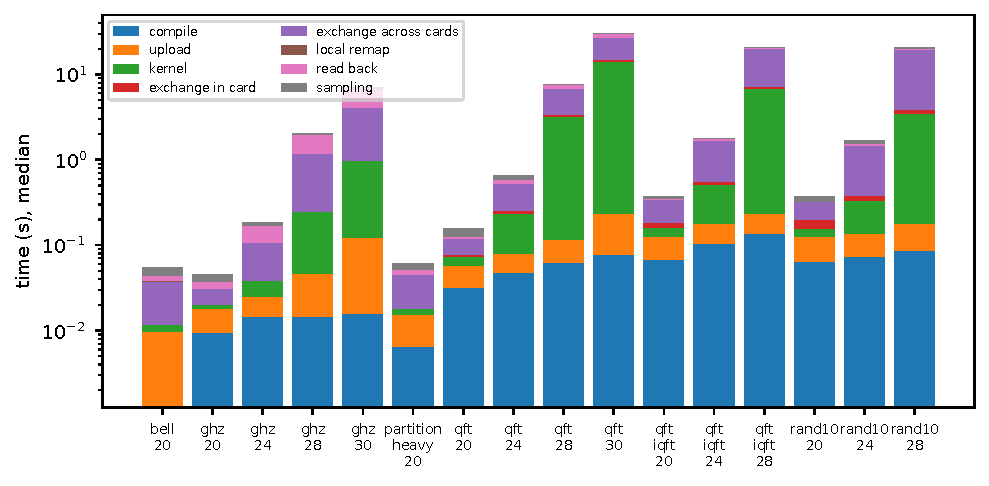
\includegraphics[width=\linewidth]{figures/fig_breakdown.pdf}
\caption{Per phase time of the engine on four cards (median of the timed repetitions).}\label{fig:breakdown}
\end{figure}

\begin{table}[t]
\caption{Baseline design on four cards: routing, bytes moved over PCIe and share of the run time per
phase (slowest card).}\label{tab:bytes}
% generated by scripts/make_tables.py, do not edit
\begin{tabular}{@{}lrrrrrrrrr@{}}
\toprule
Circuit & $n$ & local & diag. & exch. & PCIe (MiB) & kernel \% & PCIe \% & host \% & sync \% \\
\midrule
bell & 8 & 1 & 0 & 1 & 0.0 & 6 & 32 & 3 & 58 \\
bell & 14 & 1 & 0 & 1 & 1.0 & 19 & 26 & 5 & 50 \\
bell & 22 & 1 & 0 & 1 & 256.0 & 52 & 17 & 17 & 13 \\
ghz & 8 & 6 & 0 & 2 & 0.0 & 7 & 26 & 5 & 62 \\
ghz & 14 & 12 & 0 & 2 & 1.5 & 39 & 5 & 25 & 31 \\
ghz & 22 & 20 & 0 & 2 & 384.0 & 94 & 2 & 2 & 2 \\
partition heavy & 8 & 0 & 0 & 40 & 0.3 & 0 & 31 & 5 & 64 \\
partition heavy & 14 & 0 & 0 & 40 & 20.5 & 0 & 35 & 7 & 58 \\
partition heavy & 22 & 0 & 0 & 40 & 5248.0 & 0 & 48 & 26 & 27 \\
qft & 8 & 23 & 13 & 4 & 0.1 & 12 & 32 & 3 & 54 \\
qft & 14 & 83 & 25 & 4 & 15.0 & 88 & 5 & 1 & 7 \\
qft & 22 & 219 & 41 & 4 & 5888.0 & 98 & 1 & 0 & 1 \\
qft & 26 & 311 & 49 & 4 & 110592.0 & 98 & 0 & 0 & 1 \\
qft iqft & 8 & 52 & 26 & 10 & 0.3 & 11 & 31 & 4 & 54 \\
qft iqft & 14 & 178 & 50 & 10 & 30.5 & 89 & 5 & 1 & 6 \\
qft iqft & 22 & 458 & 82 & 10 & 11904.0 & 98 & 1 & 0 & 1 \\
rand10 & 8 & 81 & 10 & 29 & 0.3 & 8 & 26 & 4 & 61 \\
rand10 & 14 & 171 & 11 & 28 & 20.0 & 64 & 9 & 7 & 19 \\
rand10 & 22 & 290 & 14 & 26 & 5248.0 & 94 & 2 & 1 & 2 \\
\bottomrule
\end{tabular}

\end{table}

\begin{figure}[t]
\centering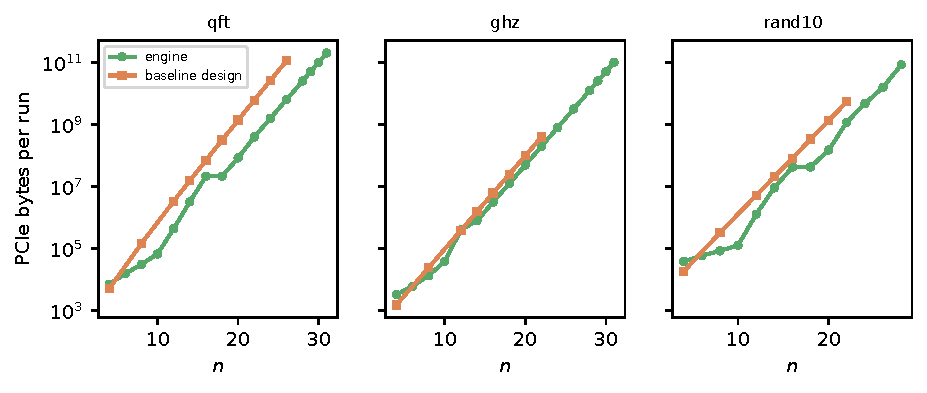
\includegraphics[width=\linewidth]{figures/fig_bytes.pdf}
\caption{PCIe bytes per run on four cards, including the state upload and read back, for the baseline design and
the engine (the engine also counts its instruction uploads).}\label{fig:bytes}
\end{figure}

\begin{table}[t]
\caption{Engine microbenchmarks on four cards, \NumEnginesFlagship~engines per card: launch of an empty segment, one
pass with one operation, and the HBM rate it implies (one read and one write of every slice), for slice widths $L$.}\label{tab:micro}
% generated by scripts/make_tables.py, do not edit
\begin{tabular}{@{}rrrrrr@{}}
\toprule
$L$ & slice (MiB) & launch (ms) & one pass (ms) & HBM, all cards (GB/s) & per card (GB/s) \\
\midrule
11 & 0.03125 & 0.79 & 0.78 & 3 & 1 \\
12 & 0.0625 & 0.79 & 0.781 & 5 & 1 \\
13 & 0.125 & 0.78 & 0.52 & 16 & 4 \\
14 & 0.25 & 1.06 & 0.593 & 28 & 7 \\
15 & 0.5 & 0.79 & 0.609 & 55 & 14 \\
16 & 1 & 0.77 & 0.689 & 97 & 24 \\
17 & 2 & 1.01 & 0.922 & 146 & 36 \\
18 & 4 & 0.77 & 1.21 & 221 & 55 \\
19 & 8 & 0.77 & 2.19 & 245 & 61 \\
20 & 16 & 0.79 & 3.61 & 298 & 74 \\
21 & 32 & 0.76 & 6.55 & 328 & 82 \\
22 & 64 & 0.83 & 12.2 & 353 & 88 \\
23 & 128 & 0.82 & 23.2 & 370 & 92 \\
24 & 256 & 1.00 & 45.3 & 379 & 95 \\
\bottomrule
\end{tabular}

\end{table}

\paragraph{HBM streaming and compute.} A pass reads and writes every slice once. With slices of $2^{\NumHbmLmax}$
amplitudes the \NumEnginesFlagship~engines of each card stream \NumHbmPerCard~GB/s per card, \NumHbmAllCards~GB/s on four
cards (Table~\ref{tab:micro}); this is the measured rate of the design, well below the 460~GB/s peak of the
HBM~\cite{amd_ds978}, and small slices are dominated by the launch time of \NumLaunchMs~ms. When a pass carries more
operations the engine becomes compute bound: each additional operation at $L=\NumPassmL$ costs \NumOpCostMs~ms, close to
the \NumOpCostModelMs~ms that follow from two amplitude pairs per cycle at \NumClockFlagship~MHz.

\paragraph{Engine.} Table~\ref{tab:routing} shows where the gates go. Of the \NumRouteQftGates~gates of the
QFT at $n=28$, \NumRouteQftLocal~run locally, \NumRouteQftFtwo~under the slice enable (F2) and \NumRouteQftFone~as slice
diagonal records (F1); the SWAP gates are absorbed into the qubit map, and only \NumRouteQftExch~gates need a remap. The
records are packed into \NumRouteQftPasses~HBM passes, so the state is swept far fewer times than there are gates. On four
cards the FPGA kernels then take \NumQftTwentyEightKernelPct\,\% of the end to end time and PCIe transfers (state
upload, exchanges across cards, read back) \NumQftTwentyEightPciePct\,\% (Fig.~\ref{fig:breakdown}); the remaining time
is compilation and host bookkeeping. The exchanges are thus the part that more cards make larger
(Section~\ref{subsec:res-scaling}).

\paragraph{Baseline design.} Table~\ref{tab:bytes} gives the same breakdown for the baseline design. For small
circuits most of its time is synchronisation of the card processes: \NumVsixQftEightSyncPct\,\% for the QFT at $n=8$,
against \NumVsixQftEightKernelPct\,\% in the kernel. From $n\approx 14$ on, its per gate kernel sweeps dominate, with
\NumVsixQftTwentyTwoKernelPct\,\% of the time at $n=22$, which is the behaviour modelled in Section~\ref{subsec:res-model}.
A circuit whose gates all act on partition qubits never reaches the kernel: the partition heavy circuit at $n=22$ spends
\NumVsixPhTwentyTwoPciePct\,\% in PCIe transfers, \NumVsixPhTwentyTwoHostPct\,\% in host arithmetic and
\NumVsixPhTwentyTwoSyncPct\,\% in synchronisation. These are the two costs that the engine removes: per gate
sweeps by packing records into passes, and host arithmetic by executing partition gates on the cards.

\subsection{Scaling over one, two and four cards}\label{subsec:res-scaling}

\begin{table}[t]
\caption{End to end time $T$ (median), speedup $S = T_1/T_C$ and parallel efficiency $E = S/C$ for $C$ cards.}\label{tab:scaling}
% generated by scripts/make_tables.py, do not edit
\begin{tabular}{@{}l@{}}
\PENDING{scaling table (E4)}
\end{tabular}

\end{table}

\begin{figure}[t]
\centering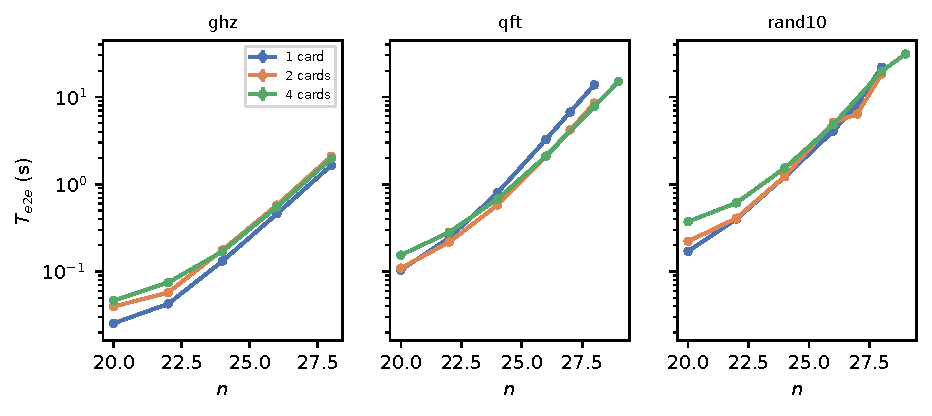
\includegraphics[width=\linewidth]{figures/fig_scaling.pdf}
\caption{End to end time on one, two and four cards (median, whiskers: interquartile range).}\label{fig:scaling}
\end{figure}

Distribution over more cards buys capacity, not speed (Table~\ref{tab:scaling}, Fig.~\ref{fig:scaling}). In
\NumScaleBelowOne~of \NumScaleCases~comparisons the two or four card run is slower than the one card run of the same
circuit. The best case is the QFT at $n=\NumScaleBestFourN$, with a speedup of \NumQftTwentyEightSpeedupTwo~on two and
\NumScaleBestFour~on four cards. The reason is the exchange path. On one card all slices share one HBM, and remaps run as
device copies, except for large remaps whose device copy chunks would be too small, which the runtime moves through host
memory. With more cards the top qubits become card qubits, and every remap that involves one of them crosses PCIe through
host memory, because peer to peer transfers between the cards are not available on this host
(Section~\ref{sec:limitations}). For the QFT at $n=28$ the exchanges take \NumScaleExchQftOne\,\% of the end to end
time on one card and \NumScaleExchQftFour\,\% on four cards, of which \NumScaleExchHostQftFour~s through the host; for the
random circuit they grow from \NumScaleExchRandOne\,\% to \NumScaleExchRandFour\,\%. The more cards hold the state,
the more of the run is PCIe traffic; with the present exchange path the four card system is the way to simulate
$n=30$ and $n=31$, not a way to simulate $n\le 29$ faster than one card. With the same number of amplitudes per card (weak scaling, $n$ on one card against $n+2$ on four), separate runs
of the QFT and the random circuit at $n=26$ and 27 on one card against $n=28$ and 29 on four cards (the four card runs
at $n=29$ are not part of Table~\ref{tab:scaling}) reach a weak scaling efficiency $T_1(n)/T_4(n+2)$ of
\NumWeakEffFourMin\,\% to \NumWeakEffFourMax\,\%, highest for the QFT and lowest for the random circuit, for the same
reason.

\subsection{Ablation of the slice paths and of the compiler rewrite}\label{subsec:res-ablation}

\begin{table}[t]
\caption{Slice paths switched off one at a time and together on two and four cards ($C$), at the largest width of the
ablation: end to end time (median) and number of remaps with all paths on and all off.}\label{tab:ablation}
% generated by scripts/make_tables.py, do not edit
\begin{tabular}{@{}l@{}}
\PENDING{ablation table (E5, E6)}
\end{tabular}

\end{table}

\begin{table}[t]
\caption{Baseline design, QFT on four cards with and without the partition diagonal path (the diagonal gates then
take the exchange path): routing, execution time, host compute and barrier time (slowest card), PCIe bytes of all cards,
and the speedup of the diagonal path (medians).}\label{tab:diag}
% generated by scripts/make_tables.py, do not edit
\begin{tabular}{@{}rlrrrrrrr@{}}
\toprule
$n$ & diagonal path & diagonal & exchanges & $T_{\mathrm{exec}}$ (s) & host compute (s) & barriers (s) & PCIe (MiB) & speedup \\
\midrule
8 & on & 13 & 4 & 0.0356 & 0.00118 & 0.0026 & 0 & 1.11 \\
 & off & 0 & 17 & 0.0394 & 0.0021 & 0.00743 & 0 &  \\
12 & on & 21 & 4 & 0.156 & 0.00194 & 0.00345 & 3 & 1.07 \\
 & off & 0 & 25 & 0.166 & 0.00403 & 0.0146 & 3 &  \\
16 & on & 29 & 4 & 3.58 & 0.0933 & 0.077 & 68 & 1.13 \\
 & off & 0 & 33 & 4.03 & 0.338 & 0.314 & 68 &  \\
18 & on & 33 & 4 & 18 & 0.136 & 0.0847 & 304 & 1.02 \\
 & off & 0 & 37 & 18.3 & 0.375 & 0.269 & 304 &  \\
20 & on & 37 & 4 & 89.9 & 0.336 & 0.119 & 1344 & 1.01 \\
 & off & 0 & 41 & 91.3 & 0.954 & 0.931 & 1344 &  \\
\bottomrule
\end{tabular}

\end{table}

\begin{figure}[t]
\centering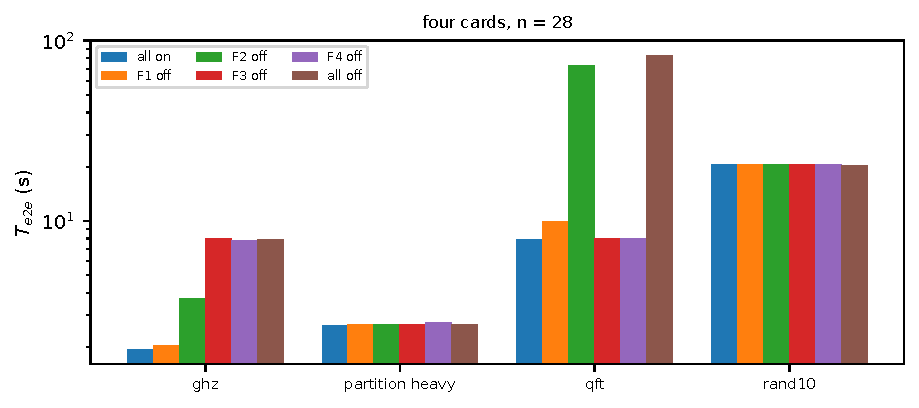
\includegraphics[width=\linewidth]{figures/fig_ablation.pdf}
\caption{End to end time of the engine on four cards with the slice paths switched off one at a time and
together, at the largest ablation width.}\label{fig:ablation}
\end{figure}

\paragraph{GHZ preparation and the compiler rewrite F4.} Three GHZ constructions were run on four cards with F4 off
and on (Section~\ref{subsec:compilation}). Without F4 the CX chain needs one remap per slice qubit,
\NumGhzChainRemapsNoFfour~at every width, and the logarithmic depth construction~\cite{cruz2019efficient} needs the same
number (\NumGhzLogRemapsNoFfour): a shorter circuit does not move fewer amplitudes. With F4 the chain needs
\NumGhzChainRemapsFfourAll~remap and the remaining CX gates become slice relabelling; at $n=28$ its end to end time falls
from \NumGhzChainTimeNoFfour~s to \NumGhzChainTimeFfour~s, a factor of \NumGhzChainSpeedupFfour~(Table~\ref{tab:ablation},
F4 off against all on). The chain rooted at the
top qubit improves by a factor of \NumGhzTopSpeedupFfour~(\NumGhzTopRemapsFfourAll~remaps), while the logarithmic
construction keeps \NumGhzLogRemapsFfourAll~remaps, because its CX targets are spread over the register. For this
hardware the useful optimisation of GHZ preparation is therefore the placement of the controls, not the depth of the
circuit.

\paragraph{Slice paths.} Table~\ref{tab:ablation} switches the slice paths off one at a time and together; a gate
whose path is off falls back to a remap. For the QFT on two cards at $n=28$ the slice controlled path F2 carries almost
the whole benefit: without it the run is \NumAblQftTwoFtwoOff~times slower, with all paths off \NumAblQftTwoAllOff~times.
Its controlled phase gates on partition qubits have a local target and a slice control, which F2 applies under the slice
enable; the slice diagonal path F1, used when the target itself is a slice qubit, adds a factor of \NumAblQftTwoFoneOff.
GHZ preparation relies on slice relabelling and the control promotion (F3, F4) and becomes \NumAblGhzTwoAllOff~times
slower without the slice paths. Grover search at $n=\NumAblGroverTwoN$ depends most on F2: its multi controlled
gates stay single records only with the slice enable (Section~\ref{subsec:compilation}); without F2 they are decomposed,
and the run is \NumAblGroverTwoFtwoOff~times slower, \NumAblGroverTwoAllOff~times with all paths off. The random circuits and the partition heavy circuit are unaffected
(\NumAblRandTwoAllOff~and \NumAblPhTwoAllOff): their slice qubits carry non diagonal single qubit gates (the random
U3 layers; H and RX in the partition heavy circuit), which need a remap with or without the slice paths, and once a slice
qubit is local the following gates on it run locally. For circuits dominated by non diagonal gates on partition
qubits the exchange path therefore sets the time. On four cards, where more gates touch slice qubits, the effects are larger: the QFT is
\NumAblQftFourFtwoOff~times slower without F2 and \NumAblQftFourAllOff~times with all paths off, GHZ
\NumAblGhzFourAllOff~times, and Grover search \NumAblGroverFourFtwoOff~times without F2.

\paragraph{Diagonal path of the baseline design.} In the baseline design a diagonal gate on a partition qubit avoids
the exchange between cards but still moves the slice of every card to the host and back, so the PCIe traffic is the
same with and without the diagonal path (\NumDiagPcieTwenty~MiB for the QFT at $n=20$, Table~\ref{tab:diag}). The path
saves host arithmetic (\NumDiagHostOffTwenty~s against \NumDiagHostOnTwenty~s at $n=20$) and barrier time
(\NumDiagBarrierOffTwenty~s against \NumDiagBarrierOnTwenty~s), but the run is dominated by the kernel sweeps of the local
gates, and the speedup of the diagonal path is only \NumDiagSpeedupMin~to \NumDiagSpeedupMax. Executing diagonal and
controlled gates on partition qubits pays off only when they run on the cards, as in the engine, where switching these
paths off makes the QFT \NumAblQftFourAllOff~times slower on four cards.

\begin{table}[t]
\caption{Choice of the partition qubits: the top qubits select the card (default) or qubits 0 and 1 do. End to end
time (median), remaps, and the ratio of the two times.}\label{tab:part}
% generated by scripts/make_tables.py, do not edit
\begin{tabular}{@{}lrrrrrrr@{}}
\toprule
 & & & \multicolumn{2}{c}{top qubits} & \multicolumn{2}{c}{qubits 0 and 1} & \\
\cmidrule(lr){4-5}\cmidrule(lr){6-7}
Circuit & $n$ & $C$ & $T_{\mathrm{e2e}}$ (s) & remaps & $T_{\mathrm{e2e}}$ (s) & remaps & ratio \\
\midrule
ghz & 16 & 2 & 0.0258 & 1 & 0.0186 & 3 & 0.72 \\
ghz & 16 & 4 & 0.0336 & 1 & 0.0581 & 4 & 1.73 \\
ghz & 20 & 2 & 0.0259 & 1 & 0.0236 & 3 & 0.91 \\
ghz & 20 & 4 & 0.0349 & 1 & 0.042 & 3 & 1.21 \\
ghz & 24 & 2 & 0.158 & 1 & 0.109 & 3 & 0.69 \\
ghz & 24 & 4 & 0.15 & 1 & 0.16 & 3 & 1.07 \\
grover & 8 & 2 & 0.0389 & 0 & 0.0372 & 1 & 0.96 \\
grover & 8 & 4 & 0.0388 & 0 & 0.0514 & 3 & 1.32 \\
grover & 12 & 2 & 0.398 & 201 & 0.401 & 201 & 1.01 \\
grover & 12 & 4 & 0.567 & 201 & 0.817 & 303 & 1.44 \\
grover & 14 & 2 & 2.62 & 803 & 3.15 & 804 & 1.20 \\
grover & 14 & 4 & 2.73 & 803 & 2.98 & 804 & 1.09 \\
qft & 16 & 2 & 0.0499 & 5 & 0.0524 & 5 & 1.05 \\
qft & 16 & 4 & 0.126 & 10 & 0.103 & 8 & 0.82 \\
qft & 20 & 2 & 0.11 & 7 & 0.105 & 6 & 0.95 \\
qft & 20 & 4 & 0.156 & 8 & 0.16 & 7 & 1.03 \\
qft & 24 & 2 & 0.576 & 8 & 0.745 & 6 & 1.29 \\
qft & 24 & 4 & 0.655 & 9 & 0.649 & 8 & 0.99 \\
\bottomrule
\end{tabular}

\end{table}

Assigning the card to qubits 0 and 1 instead of the top qubits changes the end to end time by a factor between
\NumPartRatioMin~and \NumPartRatioMax~(Table~\ref{tab:part}), and no choice is better for every circuit. The QFT acts on
all qubits alike and is nearly indifferent. GHZ needs more remaps with the low partition, because its CX chain starts at
qubit 0, yet on two cards it runs faster: all its remaps then involve engine qubits inside a card and run as device
copies, while with the top partition one remap crosses the cards through host memory. On four cards one remap still
crosses the cards, and the low partition is slower.
Grover search changes little because its oracle spans the whole register in either case. The top qubit partition is
therefore kept as the default, and the runtime accepts any initial placement.

\subsection{Comparison with Qiskit on the same host}\label{subsec:res-cpu}

\begin{table}[t]
\caption{End to end time of the FPGA system (four cards) and simulation time of Qiskit on the host CPU for the same
circuits (medians, seconds).}\label{tab:cpu}
% generated by scripts/make_tables.py, do not edit
\begin{tabular}{@{}lrrrrrr@{}}
\toprule
Circuit & $n$ & FPGA $T_{\mathrm{e2e}}$ & Statevector & Aer (all threads) & Aer (1 thread) & FPGA/Aer \\
\midrule
ghz & 12 & 0.011 & 0.000908 & 0.00172 & 0.00143 & 6.4 \\
ghz & 16 & 0.0326 & 0.0255 & 0.15 & 0.00762 & 0.22 \\
ghz & 20 & 0.0447 & 0.295 & 0.00459 & 0.135 & 9.7 \\
ghz & 22 & 0.0702 & 1.21 & 0.213 & 0.641 & 0.33 \\
ghz & 24 & 0.181 & 4.38 & 0.0867 & 2.81 & 2.1 \\
ghz & 26 & 0.555 & n/a & 0.349 & 12.2 & 1.6 \\
ghz & 28 & 2.02 & n/a & 1.31 & 52.4 & 1.5 \\
ghz & 30 & 6.98 & n/a & 5.23 & 251 & 1.3 \\
grover & 4 & 0.00854 & 0.00302 & 0.00143 & 0.00132 & 6 \\
grover & 6 & 0.0194 & 0.483 & 0.00477 & 0.00426 & 4.1 \\
grover & 8 & 0.0413 & 1.93 & 0.00681 & 0.00677 & 6.1 \\
grover & 10 & 0.0864 & 7.24 & 0.0226 & 0.0224 & 3.8 \\
grover & 12 & 0.55 & 23.8 & 0.0708 & 0.0711 & 7.8 \\
grover & 14 & 2.73 & 283 & 0.376 & 0.375 & 7.2 \\
grover & 16 & 22.7 & n/a & 0.644 & 1.66 & 35 \\
qft & 12 & 0.0216 & 0.00707 & 0.00572 & 0.00573 & 3.8 \\
qft & 16 & 0.12 & 0.554 & 0.0144 & 0.0301 & 8.3 \\
qft & 20 & 0.157 & 4.08 & 0.0296 & 0.514 & 5.3 \\
qft & 22 & 0.282 & 15.9 & 0.0654 & 2.4 & 4.3 \\
qft & 24 & 0.66 & 62.9 & 0.211 & 11.2 & 3.1 \\
qft & 26 & 2.06 & n/a & 0.88 & 50.2 & 2.3 \\
qft & 28 & 7.63 & n/a & 3.82 & 233 & 2 \\
qft & 30 & 30 & n/a & 17 & 1.15e+03 & 1.8 \\
qft iqft & 12 & 0.0392 & 0.0148 & 0.0166 & 0.0163 & 2.4 \\
qft iqft & 16 & 0.232 & 0.528 & 0.0351 & 0.0601 & 6.6 \\
qft iqft & 20 & 0.368 & 8.25 & 0.0539 & 1.07 & 6.8 \\
qft iqft & 22 & 0.589 & 33 & 0.114 & 4.98 & 5.2 \\
qft iqft & 24 & 1.8 & 131 & 0.392 & 22.8 & 4.6 \\
qft iqft & 26 & 6.3 & n/a & 1.84 & 104 & 3.4 \\
qft iqft & 28 & 20.8 & n/a & 7.21 & 481 & 2.9 \\
rand10 & 12 & 0.0495 & 0.0118 & 0.0109 & 0.0114 & 4.5 \\
rand10 & 16 & 0.275 & 0.379 & 0.0131 & 0.0401 & 21 \\
rand10 & 20 & 0.371 & 4.83 & 0.0286 & 0.696 & 13 \\
rand10 & 22 & 0.608 & 18.6 & 0.066 & 2.95 & 9.2 \\
rand10 & 24 & 1.66 & 70.3 & 0.368 & 13.7 & 4.5 \\
rand10 & 26 & 4.87 & n/a & 1.04 & 57.2 & 4.7 \\
rand10 & 28 & 20.5 & n/a & 4.38 & 252 & 4.7 \\
\bottomrule
\end{tabular}

\end{table}

\begin{figure}[t]
\centering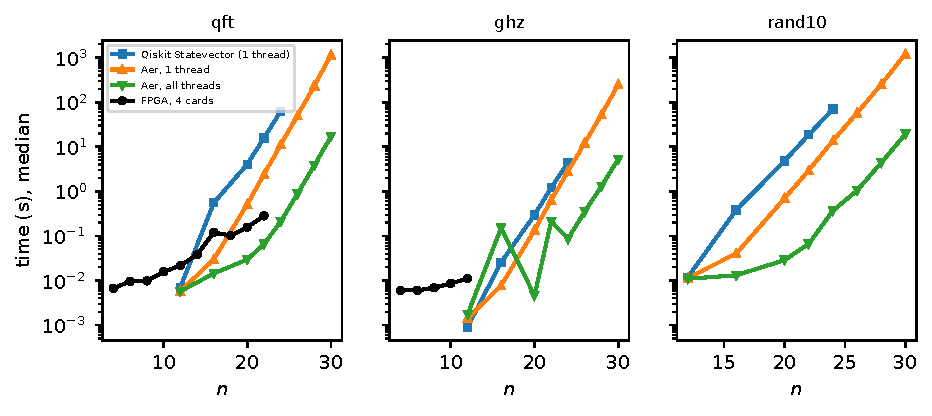
\includegraphics[width=\linewidth]{figures/fig_cpu.pdf}
\caption{End to end time of the FPGA system on four cards against Qiskit on the same host (median).}\label{fig:cpu}
\end{figure}

Qiskit Aer with all hardware threads of the \NumHostCores~core host is faster than the four card system for
almost every circuit and width (Table~\ref{tab:cpu}, Fig.~\ref{fig:cpu}): the FPGA system is faster in
\NumCpuFpgaFaster~of \NumCpuCases~cases, both GHZ circuits at widths where the multithreaded Aer time is irregular.
The gap narrows with the width, because the fixed costs of the FPGA system (compilation, launches, transfers) are
amortised and its time is set by HBM passes and exchanges: for the QFT the FPGA system is \NumCpuRatioQftSixteen~times
slower than Aer at $n=16$ and \NumCpuRatioQft~times slower at $n=30$; for GHZ at $n=30$ the factor is \NumCpuRatioGhz.
Against a single CPU thread the FPGA system is faster in \NumCpuFasterThanAerOne~of \NumCpuAerOneCases~cases and by
\NumCpuAerOneOverQft~times for the QFT at $n=30$. Grover search is the least favourable case: each iteration contains two
multi controlled gates over the whole register, which bring different qubits into the cards in turn, so that at $n=16$
the \NumGroverSixteenIters~iterations need \NumGroverSixteenRemaps~remaps, the exchanges take \NumGroverSixteenExchPct\,\%
of the end to end time, and the four card system is \NumCpuRatioGroverSixteen~times slower than Aer. We therefore make no claim of speed advantage over a multithreaded CPU
simulator on this host; the comparison with GPUs on the same card type is in the companion paper~\cite{tiwari2026fpga30}.

\subsection{Dependence on the host}\label{subsec:res-host}

\begin{table}[t]
\caption{End to end time (median, seconds) with the host process and its workers restricted to the first $N$ hardware
threads (logical CPUs $0$ to $N-1$) of the \NumHostCores~core, \NumHostThreads~thread host.}\label{tab:host}
% generated by scripts/make_tables.py, do not edit
\begin{tabular}{@{}l@{}}
\PENDING{host core table (E10)}
\end{tabular}

\end{table}

Restricting the engine runtime to between \NumHostCoresMin~and \NumHostCoresMax~hardware threads changes its end to
end time by at most \NumHostSpreadEnginePct\,\% on two and four cards, without a trend over the number of cores; the
largest spreads belong to runs of a few tenths of a second (Table~\ref{tab:host}). The runtime is one process whose
work is compilation, launches and transfers, and the gate arithmetic runs on the cards. The \NumHostCores~cores of our
host are therefore not needed: \NumHostCoresMin~hardware threads give the same times. A smaller host still needs one PCIe slot per
card and host memory for the exchanged half slices; other hosts were not measured.
The baseline design varies by \NumHostSpreadBaselinePct\,\% under the same restriction: its QFT time is spent
in the kernel sweeps of Section~\ref{subsec:res-model}, and its host arithmetic for the gates on partition qubits is a
small part of the run.

\subsection{A model of the baseline design}\label{subsec:res-model}

\begin{table}[t]
\caption{Baseline design, QFT on four cards: routing counters, measured execution time (median) and the time
predicted from microbenchmarks alone (no fitted parameter).}\label{tab:model}
% generated by scripts/make_tables.py, do not edit
\begin{tabular}{@{}rrrrrrrr@{}}
\toprule
$n$ & sweeps & launches & slice transfers & measured (s) & model (s) & model/measured & sweeps (\%) \\
\midrule
4 & 9 & 2 & 9 & 0.0179 & n/a & n/a & n/a \\
8 & 123 & 7 & 17 & 0.0345 & 0.0219 & 0.63 & 3 \\
12 & 349 & 2 & 25 & 0.155 & 0.148 & 0.96 & 82 \\
14 & 504 & 13 & 29 & 0.692 & 0.74 & 1.07 & 94 \\
16 & 687 & 15 & 33 & 3.5 & 3.82 & 1.09 & 98 \\
18 & 898 & 17 & 37 & 17.8 & 19.5 & 1.09 & 99 \\
20 & 1137 & 19 & 41 & 89.2 & 97.5 & 1.09 & 100 \\
22 & 1404 & 21 & 45 & 440 & 480 & 1.09 & 100 \\
24 & 1699 & 23 & 49 & 2.13e+03 & 2.32e+03 & 1.09 & 100 \\
26 & 2022 & 25 & 53 & 1.02e+04 & 1.11e+04 & 1.08 & 100 \\
\bottomrule
\end{tabular}

\end{table}

\begin{figure}[t]
\centering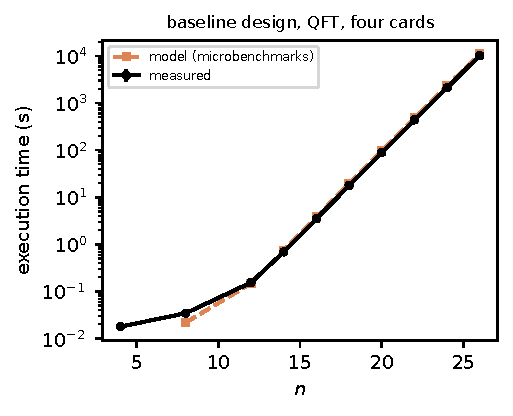
\includegraphics[width=0.6\linewidth]{figures/fig_model.pdf}
\caption{Baseline design, QFT on four cards: measured execution time and the microbenchmark model.}\label{fig:model}
\end{figure}

The timing curve of the baseline design is nearly flat for small widths and then turns upward. To explain the bend, the model of Table~\ref{tab:model}
uses only microbenchmarks of the baseline kernel on the same cards
(one launch, one gate, collection and distribution of a slice, command round trip and barrier) and the native operation
counts of each circuit, obtained by replaying the routing and the lowering of the baseline host (and checked against
the counters recorded on the cards); the relative cost of single qubit, CX and CZ operations follows from the loop
bounds and initiation intervals of the kernel source. No parameter is fitted to the circuit timings. For $n\ge 12$ the
model predicts the measured QFT time to within a factor of \NumModelRatioMin~to \NumModelRatioMax~(Fig.~\ref{fig:model}).
The QFT at $n=20$ on four cards appears in several campaigns of the baseline design (Tables~\ref{tab:model},
\ref{tab:diag} and~\ref{tab:host}); the values differ by the variation between campaigns and by whether the execution
time or the end to end time is quoted, and every comparison in the text takes both of its values from the same campaign.

The bend has a simple origin. The baseline kernel sweeps the whole slice for every native operation, and the time of a
sweep doubles with every qubit: \NumVsixSweepMsTen~ms for a slice of $2^{10}$ amplitudes and \NumVsixSweepMsSixteen~ms for
$2^{16}$, i.e.\ $t_0 = \NumVsixNsPerAmp$~ns per amplitude, or \NumVsixCyclesPerAmp~cycles of the
\NumClockVsix~MHz kernel clock. The fixed costs do not grow with the width up to slices of about $2^{14}$ amplitudes: a
kernel launch (\NumVsixLaunchMsTen~ms), the transfer of a slice to the host and back (\NumVsixXferMsTen~ms at
$2^{10}$ amplitudes), a command round trip between the host processes (\NumQueueRttUs~$\mu$s) and a barrier
(\NumBarrierUs~$\mu$s); they are set by PCIe, the XRT runtime and the host. With $W$ weighted native operations,
$N_L$ launches, $N_X$ slice transfers and $N_E$ exchanges (Table~\ref{tab:model}), the model reads
\begin{equation}
T(n) \approx W\,t_0\,2^{n_\ell} + N_L\,(t_L + t_q) + N_X\,(t_X + t_q) + 3N_E\,t_b, \qquad n_\ell = n - \log_2 C,
\label{eq:model}
\end{equation}
and the bend lies where the first term equals the sum of the others,
\begin{equation}
n^\ast = \log_2 C + \log_2 \frac{N_L\,(t_L + t_q) + N_X\,(t_X + t_q) + 3N_E\,t_b}{W\,t_0}.
\label{eq:bend}
\end{equation}
With the counts of the QFT for $n=8$ to 16 on four cards, Eq.~\eqref{eq:bend} gives $n^\ast$ between
\NumModelNstarMin~and \NumModelNstarMax. The measured runs agree: the sweeps take \NumModelSweepShareEight\,\% of the model
time at $n=8$ and more than half from $n=\NumModelCrossN$ on, after which the curve follows the exponential growth of the
sweeps, multiplied by the number of native operations, which grows with $n$ as well. The bend is therefore set by the
ratio of the per amplitude sweep time of the kernel to the fixed costs of PCIe and the host, both measured on the
platform; a faster kernel (smaller $t_0$) moves it to larger $n$, a faster host path to smaller $n$.

\subsection{Energy}\label{subsec:res-energy}

\begin{table}[t]
\caption{Board energy per simulation: time weighted mean of the board power of every used card (XMC sensors, about
one reading per second) times the end to end time. The last column is the smallest number of sensor readings
inside one run.}\label{tab:energy}
% generated by scripts/make_tables.py, do not edit
\begin{tabular}{@{}l@{}}
\PENDING{energy table (E11)}
\end{tabular}

\end{table}

During the simulations the four cards draw together between \NumEnergyPowerMinFour~and \NumEnergyPowerMaxFour~W of
board power (Table~\ref{tab:energy}). The lowest readings of the same stage, taken while the cards wait parked
between runs, add up to \NumEnergyIdleFour~W, so about two thirds of the power is static, and the energy of a
simulation follows its run time: a QFT at $n=28$ on four cards takes \NumEnergyQftTwentyEightFour~J. The card sensors
refresh about once per second, so for runs of a few seconds the power is the time weighted mean of the readings in force during the run (zero to three new ones);
the table gives the number of readings inside the shortest run. Host power is not included because the CPU energy
counters of this host are readable only with administrator rights. Since the power grows with every card and the run time does not fall in proportion
(Section~\ref{subsec:res-scaling}), the energy of a simulation rises with the number of cards: the QFT at $n=28$
takes \NumEnergyQftTwentyEightOne~J on one card, \NumEnergyQftTwentyEightTwo~J on two and
\NumEnergyQftTwentyEightFour~J on four. For widths that fit one card, one card is the most energy efficient
configuration of this system.
